\documentclass[conference]{IEEEtran}

\usepackage{cite}

\ifCLASSINFOpdf
  \usepackage[pdftex]{graphicx}
  % declare the path(s) where your graphic files are
  \graphicspath{{../pdf/}{../jpeg/}}
  % and their extensions so you won't have to specify these with
  % every instance of \includegraphics
  \DeclareGraphicsExtensions{.pdf,.jpeg,.png}
\else
  % or other class option (dvipsone, dvipdf, if not using dvips). graphicx
  % will default to the driver specified in the system graphics.cfg if no
  % driver is specified.
  % \usepackage[dvips]{graphicx}
  % declare the path(s) where your graphic files are
  % \graphicspath{{../eps/}}
  % and their extensions so you won't have to specify these with
  % every instance of \includegraphics
  % \DeclareGraphicsExtensions{.eps}
\fi

% *** SPECIALIZED LIST PACKAGES ***
%
\usepackage{algorithmic}
\usepackage{algorithm}

%
\usepackage{url}

% correct bad hyphenation here
\hyphenation{op-tical net-works semi-conduc-tor}


\begin{document}
%
% paper title
% can use linebreaks \\ within to get better formatting as desired
\title{SoNIC over 1G}


% author names and affiliations
% use a multiple column layout for up to three different
% affiliations
\author{\IEEEauthorblockN{Adithya Venkatesh, Nandini Nagaraj, Rafael Farias Marinheiro and Han Wang}
\IEEEauthorblockA{
Cornell University}
}

\maketitle


\begin{abstract}
%\boldmath

In standard environments, both Data Link and the Physical (PHY) layers are defined in the Network Interface Cards (NIC) and they cannot be accessed in real-time via software. However, these lower layers contain valuable information that can be used to measure and to improve the performance of the network. Recently, SoNIC \cite{lee2013sonic} was proposed to provide real-time access to the Physical Layer and it was used to accurately measure the performance of a high-speed wired complex network \cite{wang2014timing}. Current SoNIC design and implementation only operates in 10 GbE (Gigabit Ethernet) devices. In this project, we present a SoNIC design for 1GbE devices, extending the SoNIC ecosystem.

\end{abstract}

\IEEEpeerreviewmaketitle

\section{Introduction}

In standard environments, both Data Link and the Physical (PHY) layers are defined in the Network Interface Cards (NIC) and they cannot be accessed in real-time via software. However, these lower layers contain valuable information that can be used to measure and to improve the performance of the network. Recently, SoNIC \cite{lee2013sonic} was proposed to provide real-time access to the Physical Layer and it was used to accurately measure the performance of a high-speed wired complex network \cite{wang2014timing}. However, current SoNIC design and implementation only operates in 10 GbE (Gigabit Ethernet) devices. 

\section{Background}

Duis dictum malesuada arcu, ut tempor arcu tempus finibus. Proin posuere fringilla ullamcorper. Aenean sit amet eros odio. Pellentesque tristique facilisis placerat. Phasellus aliquam id nisl in ultricies. Pellentesque mattis suscipit nisl et ullamcorper. Pellentesque porta, justo ut dignissim rutrum, ante ante consectetur odio, a placerat sapien massa in erat. Nam blandit ultrices euismod. Vestibulum et magna rhoncus, fringilla sem vitae, hendrerit tortor. Nullam tincidunt purus ac est tempor ullamcorper.

\subsection{Hardware}

Quisque eget metus id massa pulvinar laoreet sit amet nec ligula. Donec feugiat lacus id mauris convallis, quis vehicula odio rutrum. Aliquam dictum mauris in nisi tristique suscipit. Nulla ullamcorper pellentesque dui, elementum congue tortor lacinia dignissim. In rutrum id justo id euismod. Curabitur varius diam lorem, nec mollis nibh maximus ut. Vestibulum malesuada dui convallis massa dictum, vel euismod tellus hendrerit. Etiam vitae urna faucibus, mattis tellus sed, scelerisque ante. Sed vel lectus convallis, egestas ante ut, laoreet dui. Sed iaculis arcu non auctor dignissim. Donec efficitur est a nunc accumsan cursus. Nulla orci erat, placerat eu erat vel, ultricies molestie magna. Quisque eleifend lacus vel urna ullamcorper imperdiet. Vestibulum in odio a tellus porttitor malesuada.

\section{Related Work}

Duis dictum malesuada arcu, ut tempor arcu tempus finibus. Proin posuere fringilla ullamcorper. Aenean sit amet eros odio. Pellentesque tristique facilisis placerat. Phasellus aliquam id nisl in ultricies. Pellentesque mattis suscipit nisl et ullamcorper. Pellentesque porta, justo ut dignissim rutrum, ante ante consectetur odio, a placerat sapien massa in erat. Nam blandit ultrices euismod. Vestibulum et magna rhoncus, fringilla sem vitae, hendrerit tortor. Nullam tincidunt purus ac est tempor ullamcorper.

Quisque eget metus id massa pulvinar laoreet sit amet nec ligula. Donec feugiat lacus id mauris convallis, quis vehicula odio rutrum. Aliquam dictum mauris in nisi tristique suscipit. Nulla ullamcorper pellentesque dui, elementum congue tortor lacinia dignissim. In rutrum id justo id euismod. Curabitur varius diam lorem, nec mollis nibh maximus ut. Vestibulum malesuada dui convallis massa dictum, vel euismod tellus hendrerit. Etiam vitae urna faucibus, mattis tellus sed, scelerisque ante. Sed vel lectus convallis, egestas ante ut, laoreet dui. Sed iaculis arcu non auctor dignissim. Donec efficitur est a nunc accumsan cursus. Nulla orci erat, placerat eu erat vel, ultricies molestie magna. Quisque eleifend lacus vel urna ullamcorper imperdiet. Vestibulum in odio a tellus porttitor malesuada.

\section{Design}

Duis dictum malesuada arcu, ut tempor arcu tempus finibus. Proin posuere fringilla ullamcorper. Aenean sit amet eros odio. Pellentesque tristique facilisis placerat. Phasellus aliquam id nisl in ultricies. Pellentesque mattis suscipit nisl et ullamcorper. Pellentesque porta, justo ut dignissim rutrum, ante ante consectetur odio, a placerat sapien massa in erat. Nam blandit ultrices euismod. Vestibulum et magna rhoncus, fringilla sem vitae, hendrerit tortor. Nullam tincidunt purus ac est tempor ullamcorper.

Quisque eget metus id massa pulvinar laoreet sit amet nec ligula. Donec feugiat lacus id mauris convallis, quis vehicula odio rutrum. Aliquam dictum mauris in nisi tristique suscipit. Nulla ullamcorper pellentesque dui, elementum congue tortor lacinia dignissim. In rutrum id justo id euismod. Curabitur varius diam lorem, nec mollis nibh maximus ut. Vestibulum malesuada dui convallis massa dictum, vel euismod tellus hendrerit. Etiam vitae urna faucibus, mattis tellus sed, scelerisque ante. Sed vel lectus convallis, egestas ante ut, laoreet dui. Sed iaculis arcu non auctor dignissim. Donec efficitur est a nunc accumsan cursus. Nulla orci erat, placerat eu erat vel, ultricies molestie magna. Quisque eleifend lacus vel urna ullamcorper imperdiet. Vestibulum in odio a tellus porttitor malesuada.

\section{Implementation}

\subsection{8b10b Codec}

1G SoNIC requires an 8b10b encoder/decoder to be available to the Physical Coding Sublayer (PCS). The 8b10b encoder converts an 8-bit input into a 10-bit output, the decoder does the opposite. Valid inputs to the codec are available in the \cite{ieee8023}, and each 80bit input maps to one of two 10-bit outputs depending on the running disparity of the codec (difference between the number of set and unset bits in each input to the encoder).The 8b10b Codec for 1G SoNIC is implemented in C. The software implementation functions as below. It has two 3/4 lookup tables and two 5/6 lookup tables, one for the positive running disparity and the other for the negative running disparity, containing 8 and 32 entries respectively. The decoder works with a reverse lookup table and does not have to keep track of the running disparity.

\begin{figure}[h!]
  \centering
  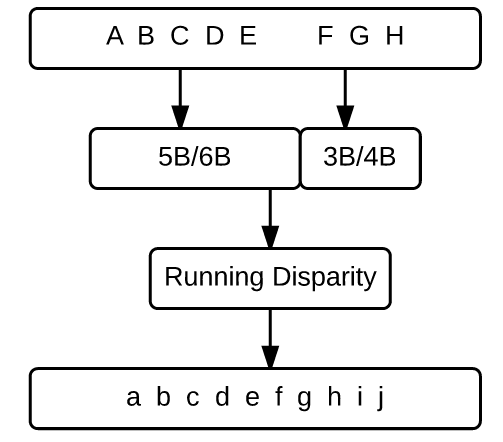
\includegraphics[scale=0.50]{encoder}
  \caption{Encoder}
  \label{fig:encoder}
\end{figure}

Decoding happens between the PCS and the Gigabit Media Independent Interface (GMII). Encoding happens between the PCS and the Physical Medium  Attachment (PMA). The codec is required to allow the clock to recover between states. This relaxation is provided by adding the 2 extra bits which increase the time required to process by 25\%.

While the implementation was straight-forward it was necessary to ensure that the codec adhered to the 1Gbps line-rate of the device. The initial implementation used the right shift operator in C to count the number of bits set to 1 in the 8-bit input, however this proved to be too computationally expensive to let the codec meet the 1Gbps line-rate. The builtin popcount method, provided by GCC combined with compiler optimizations, proved to be the key for efficient computation of the number of bits in the input byte and let the program meet the line-rate requirements.

\section{Evaluation}

The 8b10b codec was evaluated to measure the rate at which it processes data and to ensure that it met the 1Gbps requirement. The encoder takes an 8-bit input, 1Gb is $1024^3 = 1073741824bits$ and is the same as $134217728 x$ 8-bit inputs. An encoder that meets the line-rate requirement would process this amount of data withing a 1 second window. In the same vein, a decoder that performs at line-rate would process $107374183 x $ 10-bit inputs within this 1 second. The encoder and decoder were both tested for varying input sizes in increments of 1Gb for each test and the results are visible below.

\begin{figure}[h!]
  \centering
  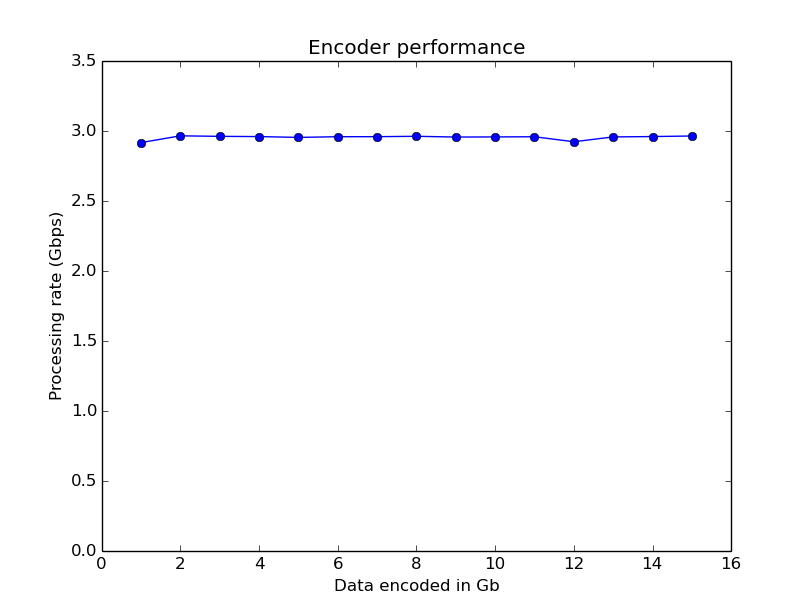
\includegraphics[scale=0.50]{encoder_figure}
  \caption{Encoder Performance}
  \label{fig:encoder_performance}
\end{figure}

\begin{figure}[h!]
  \centering
  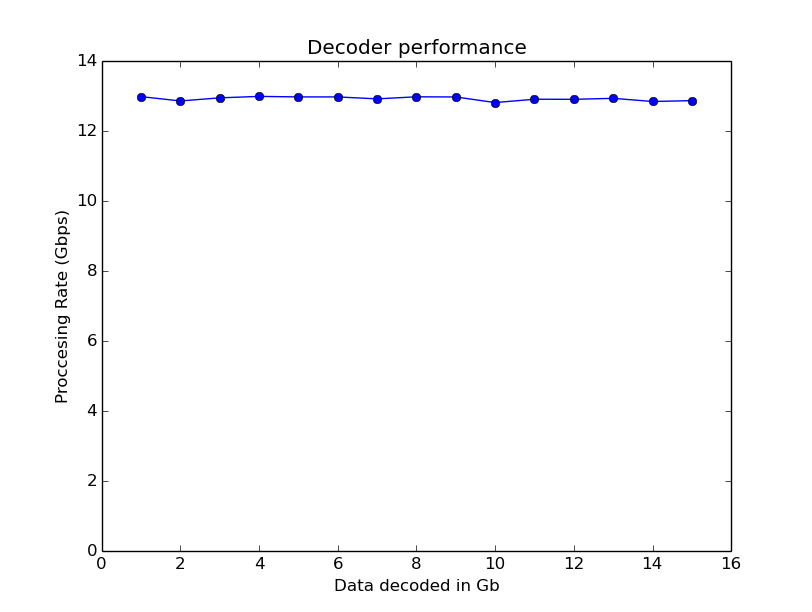
\includegraphics[scale=0.50]{decoder_figure}
  \caption{Decoder Performance}
  \label{fig:decoder_performance}
\end{figure}

\subsection{Correctness}


\section{Conclusion}

Quisque eget metus id massa pulvinar laoreet sit amet nec ligula. Donec feugiat lacus id mauris convallis, quis vehicula odio rutrum. Aliquam dictum mauris in nisi tristique suscipit. Nulla ullamcorper pellentesque dui, elementum congue tortor lacinia dignissim. In rutrum id justo id euismod. Curabitur varius diam lorem, nec mollis nibh maximus ut. Vestibulum malesuada dui convallis massa dictum, vel euismod tellus hendrerit. Etiam vitae urna faucibus, mattis tellus sed, scelerisque ante. Sed vel lectus convallis, egestas ante ut, laoreet dui. Sed iaculis arcu non auctor dignissim. Donec efficitur est a nunc accumsan cursus. Nulla orci erat, placerat eu erat vel, ultricies molestie magna. Quisque eleifend lacus vel urna ullamcorper imperdiet. Vestibulum in odio a tellus porttitor malesuada.

\bibliographystyle{IEEEtran}
\bibliography{report}

\end{document}